\documentclass[oneside]{book}
\usepackage{xcolor}
\definecolor{bg}{rgb}{0.95,0.95,0.95}
\definecolor{emphcolor}{rgb}{0.5,0.0,0.0}
\newcommand{\empha}{\bf\color{emphcolor}}
\usepackage{parskip}
\usepackage{minted}
\usepackage{caption}
\usepackage{amsmath}
\usepackage{amssymb}
\usepackage{amscd}
\usemintedstyle{friendly}
\setminted{bgcolor=bg,xleftmargin=15pt}
\usepackage{hyperref}
\hypersetup{pdftex,colorlinks=true,allcolors=blue}
\usepackage{hypcap}
\usepackage{graphicx}
\title{Communicating Sequential Processes\\ in C++}
\author{John Skaller}
\begin{document}
\maketitle
\tableofcontents
\chapter{CSP model}
The CSP kernel supports a simple architecture.

\section{Systems}
A {\em system} consists of several {\em processes} which communicate
using {\em asynchronous channels}. Systems are used to manage 
core {\em internal} resources: processing elements (CPUs), program code,
time, and data memory.

A {\em device} is an arbitrary object and associated service thread which is
used to manage {\em external} resources, including network and file system access,
and user interfaces.


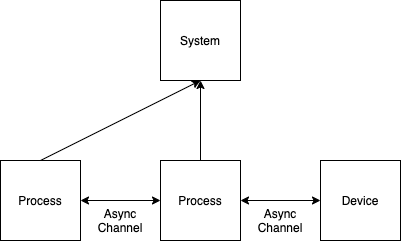
\includegraphics{../src/tex/system.png}

Processes within the same system can communicate with each other or
with devices. Processes in distinct systems must use a device as
a middleman to communicate.

\section{Processes}
The execution of a process is effected by one or more {\em threads}.
If there is only one, the process is {\em single threaded,} otherwise
if there are two or more, {\em multi-threaded.} Every process is started
with a single {\em initial} thread.

A {\em fibre} is a logical thread of control and associated execution
context. Each process consists of a collection of fibres. 

Fibres in a process are {\em running} if a thread is elaborating the
fibre's program code, otherwise the fibre is {\em suspended}. 

A suspended fibre can either be {\em ready} or {\em waiting}.
The collection of ready and running fibres are said to be {\em active}.

All the ready fibres of a processes are maintained in a set and
are owned by their process. Running fibres are owned by the thread
running them which are owned by the thread's process.

When a thread is out of work, it attempts to locate a 
ready fibre then run it. If there are no ready fibres,
no fibres are running, and there are no fibres waiting on
asynchronous I/O from an external device or another system,
then the process terminates and all associated memory is released,
all but the initial thread are terminated, and the initial thread
returns control.

A process is initiated by a single C++ function call
which is passed a pointer to the initial continuation to invoke
and a pointer to the owning system. A single threaded processes
is then constructed with a single fibre owning the initial 
continuation.

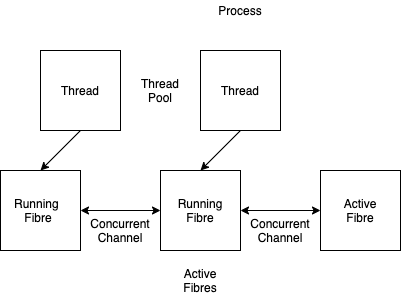
\includegraphics{../src/tex/process.png}


\section{Fibres}

A {\em fibre} consists of a stack of continuations.

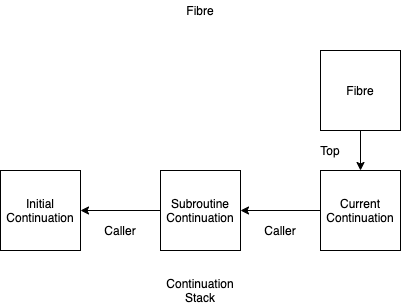
\includegraphics{../src/tex/fibre.png}

\section{Channels}

A {\em channel} is a synchronisation primitive which also allows transmission
of data.\

Channels are accessed via {\em channel endpoints}, using {\em channel endpoint references.}

A particular channel enpoint may be accessed only from the continuations
of one fibre; that is, each endpoint must be uniquely owned by a single
fibre. This invariant ensures the correct termination of fibres
making I/O requests which cannot be satisfied. 

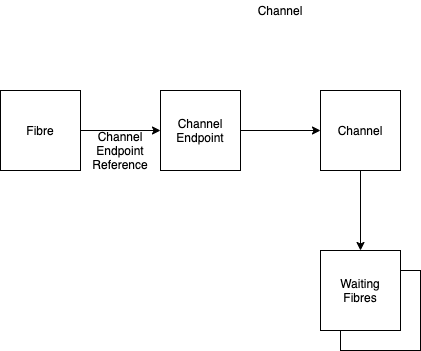
\includegraphics{../src/tex/channel.png}

\chapter{Access}
Objects in the system can access others using either pointers
or reference counting smart pointers. A variable containing a pointer
which expresses ownership is called a {\em strong pointer variable}.
Reference counting pointer variables are always strong.

Ordinary pointers can also be strong. In this case, the object referred
to must be manually deleted before the object containing the variable
is destroyed.

A weak pointer variable is a variable containing a pointer which provides
access to an object which owns, directly or indirectly, the containing
variable. Such objects must be deleted before the owning object is deleted
so that the lifetime of the weak pointer variable is contained temporally
in the owner lifetime.

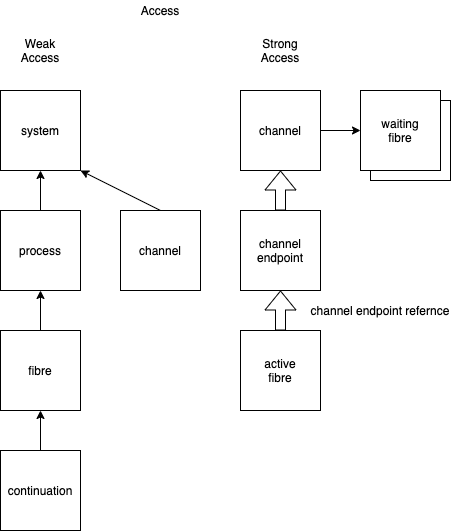
\includegraphics{../src/tex/weak_access.png}

\chapter{Operational Semantics}
The core semantic operations of the system are construction of
processes, threads, and fibres, and channel I/O.

Reads and writes on channels are performed with special service calls
which are given a channel endpoint reference. The semantic rules
are simple enough.

A channel may be in three states. It may be empty, consist of a set
of readers, or consist of a set of writers.

When a write is performed then, if the channel is empty or consists 
of a set of writers, the fibre performing the write is added to the channel.
Since this fibre we the currently running fibre of some thread, and the
fibre is now suspended, the thread no attempts to find another 
fibre to execute.

If the channel contains a reader then, instead, it is removed from
the channel. Data is transfered from the writer to the reader.
Nominally, both fibres then become active fibres of their 
respective processes.


\chapter{Allocators}
An {\em allocator} is an object with two methods, \verb$allocate$ and 
\verb$deallocate$, used to manage memory blocks. The allocate method
retrieves an available block of a particular size, and the deallocate
method returns to the free store.

Each system has a {\em system allocator} which must be used to construct
process objects, channel objects, and channel endpoint objects.

Each process has a {\em process allocator} which must be used to construct
fibres and continuations of that process.

We provide a standard system allocator of class \verb$system_allocator_t$.
This allocator is thread safe and uses spinlocks to protect the
allocation and deallocation methods. 

The management objects and the user memory blocks are all suballocated 
from a single large memory block retrieved from another allocator, 
its {\em bootstrap allocator.}  We provide a convenience allocator
which can be used as the initial bootstrap for other allocators,
of class \verb%malloc_free_t% allocator.

The standard system allocator requires that only blocks retrieved
from it by \verb%allocate% be returned to it, by method \verb$deallocte$.
In addition, no more than the available number of blocks of any particular
size may be allocated or the behaviour is undefined. The system allocator
must be constructed with the maximum number of blocks required.

Requests for a particular size are mapped to requests for the size which
is the innitially specified size which is the least upper bound of the
requested size. Requests for blocks larger than any specified size
have undefined behaviour.

The model is based on the fact that all programs are ultimately
finite state machines. This requires all scalable programs be bounded
so that the maximum number of blocks of any particular size ever required
at any time can be calculated and thus pre-allocated.

\section{Allocator Structures}
All allocators are used via a reference counting handle
\verb$alloc_ref_t$. Every non-root allocator has constructors
whose first argument is a handle to its parent, which is the 
allocator that constructed it. This ensure the parent remains live
whilst its child does, and provides access to the parent which
must be used to deallocate it.

A root allocator is passed a \verb%nullptr% and is created by 
\verb$C++$ standard \verb$new$ and deallocated by \verb$delete$.
Therefore, allocators must form a directed acyclic graph with respect
to parentage.

In addition many allocators delegate to others, often one other,
but many others could be used. The delegation graph must also
be a directed acyclic graph.





\end{document}
